\documentclass{report}
\usepackage{graphicx}
\begin{document}

\title{Tugas Mata Kuliah Kecerdasan Buatan}
\maketitle

{\bf Muhammad Nazhim Maulana (1194025)}
\vspace{0.1cm}

{\bf Definisi Kecerdasan Buatan}
\vspace{0.1cm}
\\\hangindent=0.5cm Berdasarkan Pengertian nya kecerdasan buatan atau yang lebih dikenal dalam Bahasa Inggris sebagai \emph{Artificial Intelligence}. Secara sederhana, sebuah kecerdasan buatan itu bisa diartikan sebagai sebuah sistem kecerdasan yang manusia tanamkan ke dalam sebuah teknologi dan sistem kecerdasan ini juga bergantung terhadap banyaknya data yang di berikan. Maksudnya disini adalah semakin banyak data yang dimiliki maka akan semakin akurat juga program yang berjalan pada teknologi tersebut.

\vspace{0.5cm}

{\bf Sejarah dan Perkembangan Kecerdasan Buatan}
\vspace{0.1cm}
\\\hangindent=0.5cm Berdasarkan sejarah, istilah \emph{Artificial Intelligence} itu pertama kali ditemukan pada tahun 1956 dan sampai sekarang ini masih populer. Untuk penelitian atau riset awalnya dimulai pada tahun 1950an kemudian muncul keinginan dari Departemen Pertahanan Amerika Serikat untuk melatih komputer agar memiliki kecerdasan layaknya manusia.

\vspace{0.4cm}
\hangindent=0.5cm Kemudian terus terjadi perkembangan program AI yang dibuat oleh manusia mulai dari tahun 1959 dikeluarkan program yang dapat mengeluarkan teorema dengan menggunakan aksioma-aksioma yang ada. Perkembangan itu terus terjadi hingga sekarang ini dimana sudah banyak dilakukan pengembangan program-program yang dapat membantu kehidupan sehari-hari dari manusia.

\vspace{0.5cm}

{\bf \emph{Supervised} dan \emph{Unsupervised Learning}}
\vspace{0.1cm}
\\\hangindent=0.5cm \emph{Supervised Learning} adalah salah satu jenis dari algoritma yang digunakan untuk mengajar sebuah \emph{Machine Learning}, untuk pembelajarannya ini akan diawasi langsung oleh seorang \emph{Supervisor} atau pengawas. Algoritma ini akan memerlukan sebuah data berlabel untuk membangun model yang memiliki tingkat akurasi yang terus menerus dapat ditingkatkan.

\vspace{0.4cm}
\hangindent=0.5cm Selanjutnya ada \emph{Unsupervised Learning} yang merupakan kebalikan dari  \emph{Supervised Learning}. Jikalau \emph{Supervised Learning} itu memiliki pengawas, maka \emph{Unsupervised Learning} sendiri tidak diawasi. Dengan begitu algoritma ini cenderung lebih bebas dalam proses eksplorasi data karena tiap data yang ada tidak memiliki label sehingga lebih mudah dalam melakukan eksplorasi dan menemukan data yang tersembunyi. 

\vspace{0.5cm}

{\bf Regresi dan Klasifikasi}
\vspace{0.1cm}
\\\hangindent=0.5cm Regresi merupakan sebuah proses untuk menemukan korelasi antara variabel \emph{Dependent} dan \emph{Independent}. Regresi ini biasanya sangan membantu untuk melakukan prediksi yang bersifat \emph{Continuous} seperti prediksi Tren Pasar, atau bahkan hingga ke perkiraan cuaca juga dapat digunakan.

\vspace{0.4cm}
\hangindent=0.5cm Sedangkan klasifikasi merupakan sebuah proses untuk menemukan fungsi yang dapat membantu untuk melakukan pembagian terhadap dataset ke dalam kelas-kelas tertentu berdasarkan dengan parameter-parameter yang berbeda-beda. Biasanya sebuah program komputer akan dilatih dengan mengkategorikan data yang telah diberikan menjadi berbagai kelas yang berbeda-beda.

\vspace{0.5cm}

{\bf Dataset}
\vspace{0.1cm}
\\\hangindent=0.5cm Secara sederhana dataset itu merupakan kumpulan dari data yang berasal dari informasi-informasi yang ada pada masa lampau. Informasi yang diperoleh ini nantinya akan diolah kembali untuk menghasilkan sebuah informasi yang baru. Datset sendiri bisa diubah (baik ditambahkan, dihapus atau diperbarui baris yang ada di dalamnya)

\vspace{0.5cm}

{\bf \emph{Training Set} dan \emph{Testing Set} }
\vspace{0.1cm}
\\\hangindent=0.5cm Setelah membahas mengenai Dataset maka selanjutnya adalah bagian dari dataset yakni \emph{Training Set} dan \emph{Testing Set}. \emph{Training Set} merupakan bagian dari dataset yang dilatih untuk membuat prediksi atau fungsi lain yang nantinya akan ada di dalam sebuah \emph{Machine Learning}, biasanya dalam \emph{Training Set} ini diberikan algoritma untuk melatih sebuah mesin.

\vspace{0.4cm}
\hangindent=0.5cm Selain \emph{Testing Set}, ada juga yang namanya \emph{Test Set} yang merupakan bagian dari Dataset juga yang di tes untuk melihat tingkat ke akuratan atau bisa dikata untuk melihat performa dari mesin yang sudah dilatih menggunakan \emph{Training Set}.

\vspace{0.4cm}



\begin{enumerate}
   \item Instalasi Library Scikit Learn
   
	\hangindent=0.5cm Untuk instalasi dari scikit learn sendiri hasil nya dapat dilihat pada gambar berikut ini:
	
\begin{figure}[hbtp]
\caption{Hasil Instalasi}
\centering
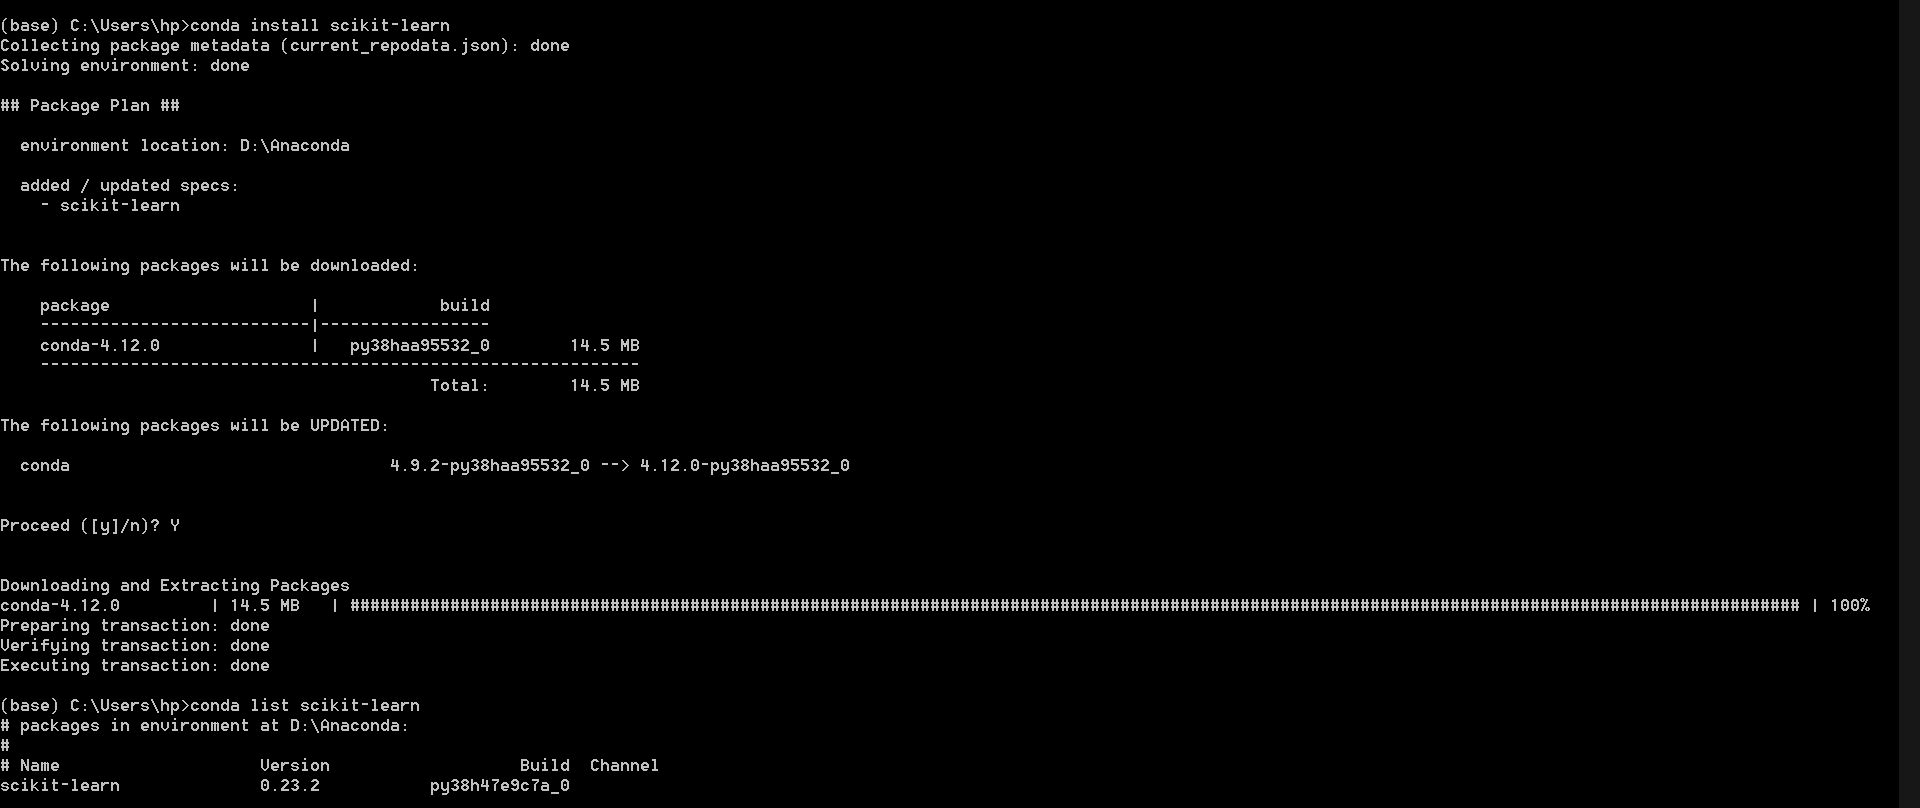
\includegraphics[scale=0.3]{../figures/1.png}
\end{figure}

	
   \item Loading Example Dataset
   
   	\hangindent=0.5cm Selanjutnya adalah loading dataset yang telah ada pada dokumentasi scikit learn maka akan diperolah beberapa hasil seperti pada gambar dibawah ini:
   	
   	\begin{figure}[hbtp]
   	\caption{Variable yang di dapatkan}
   	\centering
   	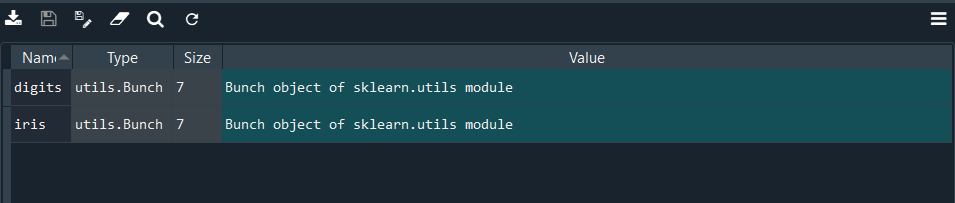
\includegraphics[scale=0.6]{../figures/Praktikum 1.png}
   	\end{figure}
   	
   \begin{figure}[hbtp]
   \caption{Hasil yang di dapatkan}
   \centering
   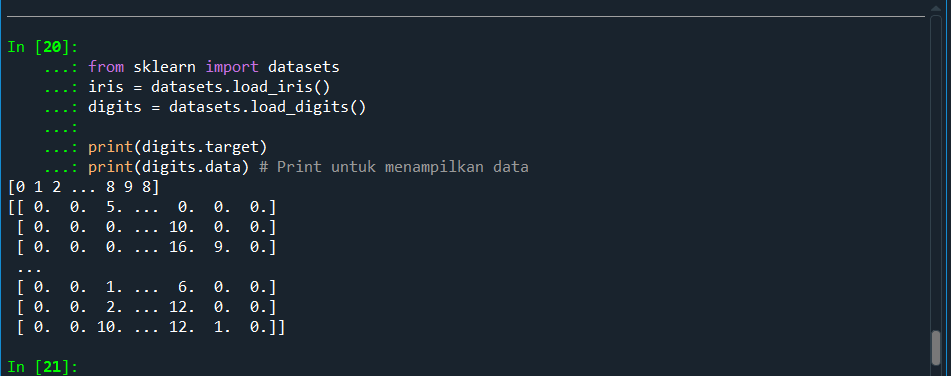
\includegraphics[scale=0.5]{../figures/Praktikum 2.png}
   \end{figure}
   
   	\hangindent=0.5cm Seperti pada gambar diatas dapat dilihat hasil yang di dapatkan untuk loading example dataset.
   	
   \item Learning and Predicting 
   
   	\hangindent=0.5cm Untuk praktikum yang selanjutnya hasil yang diperoleh adalah sebagai berikut:
   	
   	\begin{figure}[hbtp]
   	\caption{Variable yang didapatkan}
   	\centering
   	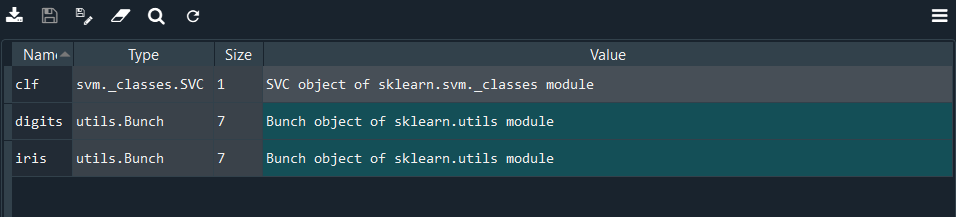
\includegraphics[scale=0.7]{../figures/Praktikum 3.png}
   	\end{figure}
   	
   	\hangindent=0.5cm Untuk praktikum yang kedua ini nantinya akan diperoleh hasil prediksi berdasarkan sampel dataset yang ada. Hasil yang diperoleh dari consolenya adalah sebagai berikut:
   	
   	\begin{figure}[hbtp]
   	\caption{Hasil Akhir pada Console}
   	\centering
   	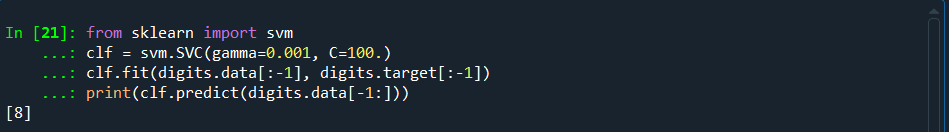
\includegraphics[scale=0.7]{../figures/Praktikum 4.png}
   	\end{figure}
   	
   \item Model Persistence
   
   	\hangindent=0.5cm Untuk praktikum yang selanjutnya hasil yang diperoleh adalah sebagai berikut untuk variabel dan juga hasil akhir pada consolenya:
   	
   	\begin{figure}[hbtp]
   	\caption{Variable yang Dihasilkan}
   	\centering
   	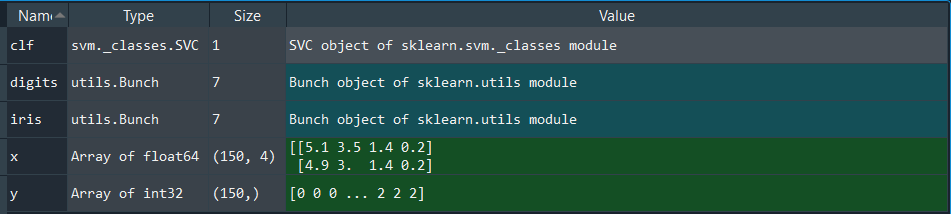
\includegraphics[scale=0.5]{../figures/Praktikum 5.png}
   	\end{figure}
   	
   	\begin{figure}[hbtp]
   	\caption{Hasil Akhir pada Console}
   	\centering
   	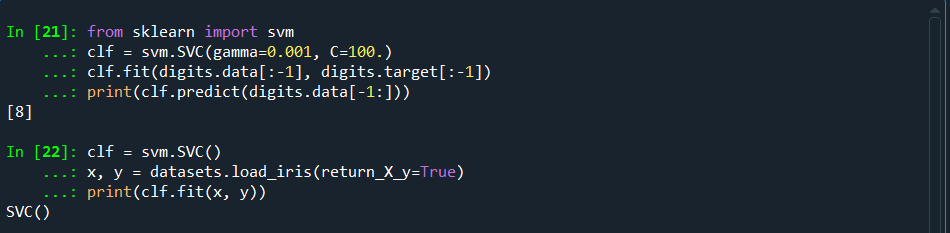
\includegraphics[scale=0.5]{../figures/Praktikum 6.png}
   	\end{figure}
   	
   \vspace{0.8cm}
   \item Conventions

   \hangindent=0.5cm Untuk praktikum yang selanjutnya hasil yang diperoleh adalah sebagai berikut untuk variabel dan juga hasil akhir pada consolenya:
   
   \begin{figure}[hbtp]
   \caption{Variable yang Di dapatkan}
   \centering
   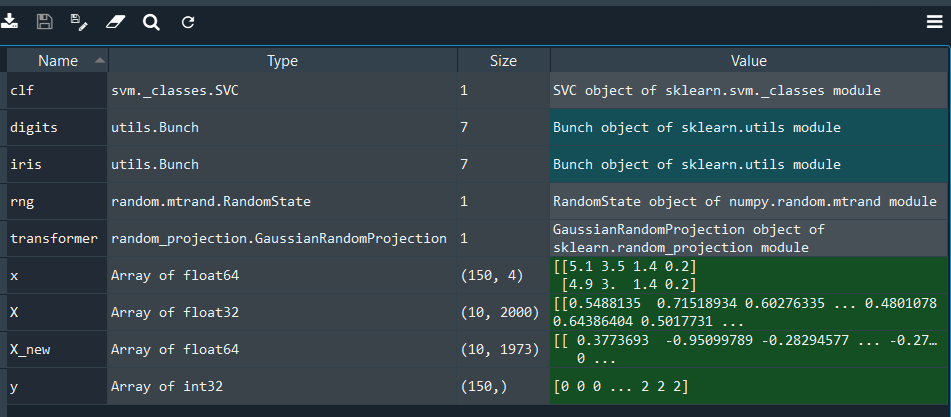
\includegraphics[scale=0.5]{../figures/Praktikum 7.png}
   \end{figure}
   
   \begin{figure}[hbtp]
   \caption{Hasil Akhir pada Console}
   \centering
   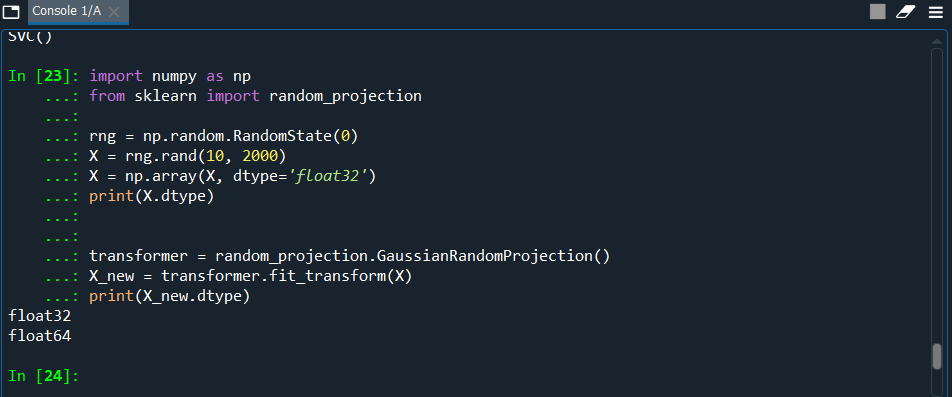
\includegraphics[scale=0.5]{../figures/Praktikum 8.png}
   \end{figure}
   
   
\end{enumerate} 


\end{document}
